\section{Generalisation}
\lecture{3}{27/1}

We need toe nsure our models are not \emph{over-fit} to the
training data and will make accurate predictions on novel data.
So how do we tell if our model is good?
Theoretically, generalisation theory is based
on ideas of measuring model simplicity and complexity.
We have the intuition of Ockham's Razor; that is,
the less compelx a model is, the more likely a good
empirical result it is (and not just due to the peculiarites of the
sample).
Empirically, we can see how well our model performs on
a new set of data. 
Good performance on this test set is a useful indicator
of good performance on new data in general as long as our
test set is large enough and we don't \emph{cheat} by reusing the
test set.

The above holds if we have the three following assumptions:
\begin{enumerate}
    \item we draw examples \emph{independently} and 
        \emph{identically} at random from the distribution;
    \item the distribution is \emph{stationary}
        (that is, it does not change over time); and
    \item we always pull from the same distribution,
        including all training, validation, and test sets.
\end{enumerate}

\section{Training and test set}

We partition our data into a training set
(used to train our mdoel)
and our test set
(used to confirm our model is good);
but how large do we make our splits for this?
If you have a larger training set then our model will
be more able to learn; 
however, if we use a larger test set
we will be able to have a higher degree in confidence in
evaluation metrics and tighter confidence intvervals.

If we only have one data set, we divide them into our training
set and test set and we \emph{do not train on the test data}.
We must ensure that the test set
\begin{enumerate}
    \item is large enough to yield statistically meaningful results; 
        and
    \item is representative of the data set as a whole.
\end{enumerate}

Figure \ref{fig:training-vs-test} illustrates an example of how
our test data is still representative of the total population,
even though there is less data.

\begin{figure}[]
    \centering
    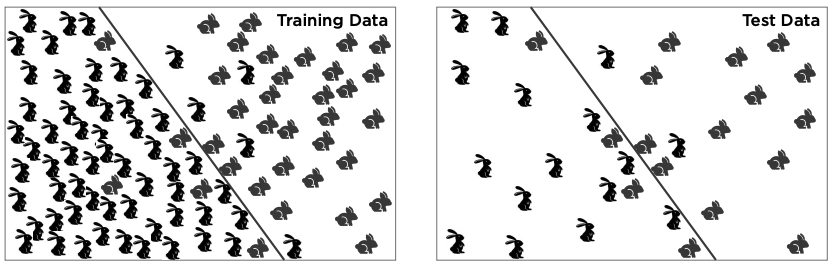
\includegraphics[width=0.8\linewidth]{images/training-vs-test.png}
    \caption{}
    \label{fig:training-vs-test}
\end{figure}

One possible workflow is to train models on a training set,
evaluating them on the test set and tweak them accordingly
(then start the process again) until we get a model that performs
the best on the test set.

A better workflow though is to introduce a \emph{validation set}.
We use this when developing our model, we train it on our
training set then evaluate it on the validation set to make tweaks.
We then pick the model that does best on the validation set and
confirm this result on the test set. 

This workflow allows us to keep the test data away from the model
throughout all of the training and creation.
It reduces the neumber of exposures to the test set and can
prevent \emph{over training}.

\section{Representation}

Our model can only see what we give it. 
We are responsible for choicing an appropriate \emph{representation}
of the data to provide the model with a useful
\emph{vantage point} into the data's important qualities.
More precisely, we need to choose a set of features that 
best represent the data (in regards to what we are trying to predict).

Say we are given the age of a person and are trying to predict
there income, we may be tempted to draw a linear relationship
such that the older you are the higher your income will be;
however, this relationship is not a simple linear regression.
It may be able to be broken down into several different linear
regressions, so we can use a technique called \emph{bucketing}.
We get a categorical feature created for each bucket.
%todo talk to jacob maybe this doesn't really make much sense.
